\documentclass[tikz,border=10pt]{standalone}
\usepackage{tikz}

\begin{document}

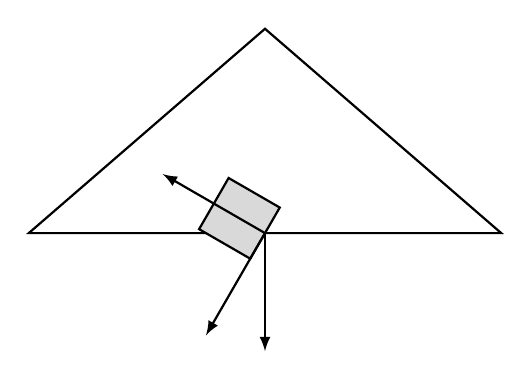
\begin{tikzpicture}[scale=1.5]
    % Draw inclined plane
    \draw[thick] (-2,0) -- (2,0) -- (0,1.73) -- cycle;

    % Draw rectangle (car) on inclined plane
    \draw[thick,rotate around={60:(0,0)},fill=gray!30] (-0.25,0) rectangle (0.25,0.5);

    % Draw forces
    % force of gravity
    \draw[thick,-latex] (0,0) -- (0,-1) node[midway,left] {};
    % normal force
    \draw[thick,-latex,rotate around={60:(0,0)}] (0,0) -- (0,1) node[midway,right] {};
    % frictional force
    \draw[thick,-latex,rotate around={60:(0,0)}] (0,0) -- (-1,0) node[midway,above] {};
\end{tikzpicture}

\end{document}